\section{Blockchain}
\label{sec:blockchain}

Blockchain adalah sekuens dari blok yang menyimpan daftar transaksi lengkap seperti \textit{public ledger} konvensional, dimana setiap \textit{ledger} disimpan pada \textit{node} yang tersebar seperti pada \textit{Distributed Ledger Technology} \parencite{zheng2018blockchain}. Setiap transaksi yang masuk ke dalam sebuah blok akan divalidasi sesuai dengan metrik yang digunakan oleh sistem Blockchain, dan blok yang memiliki daftar transaksi yang lengkap, ditambah \textit{timestamp} pembuatan blok, nilai \textit{hash} dari blok sebelumnya ("\textit{parent}"), dan sebuah \textit{nonce}, yang adalah sebuah angka acak yang digunakan untuk mekanisme verifikasi \textit{hash}. Konsep ini memastikan integritas dari Blockchain dimulai dari blok pertama ("\textit{genesis block}") sampai ke blok terakhir, yang terus ditambahkan, karena setiap perubahan data akan membuat nilai \textit{hash} dari sebuah blok berubah, yang harus dipropagasikan ke setiap blok setelahnya. Sebelum ditambahkan ke dalam Blockchain, setiap blok dan transaksi di dalamnya harus divalidasi oleh mayoritas \textit{node}, menggunakan sebuah mekanisme \textit{consensus} \parencite{nofer2017blockchain}. Mekanisme \textit{consensus} adalah proses dimana mayoritas dari \textit{network validator} menyetujui atau menolak sebuah \textit{state} dari \textit{ledger}. Proses \textit{consensus} mengikuti sebuah kumpulan aturan dan prosedur untuk mempertahankan himpunan fakta yang koheren diantara beberapa \textit{participating nodes}. Terdapat banyak mekanisme \textit{consensus} yang berbeda yang digunakan dalam \textit{Blockchain network} yang berbeda. Dalam kasus \textit{Bitcoin}, \textit{ledger} yang dianggap \textit{ledger} yang \textit{valid} adalah \textit{ledger} dengan \textit{chain} terpanjang (\textit{longest chain}) \parencite{swanson2015consensus}.

\begin{figure}[ht]
	\centering
	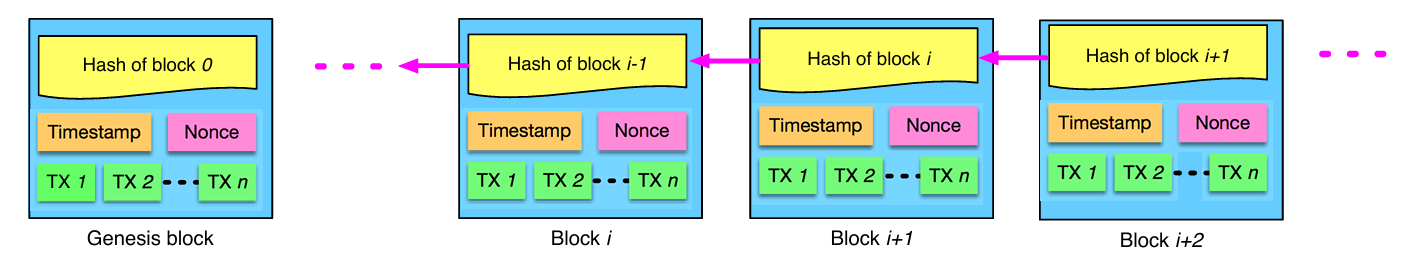
\includegraphics[width=1\textwidth]{resources/chapter-2/struktur-blockchain.png}
	\caption{Struktur blok di dalam Blockchain \parencite{zheng2018blockchain}}
	\label{image:struktur-blockchain}
\end{figure}

\break

Struktur dari sebuah blok terdiri dari \textit{block header} dan \textit{block body} seperti pada Gambar \ref{image:struktur-blok}. Secara spesifik, \textit{block header} terdiri dari:

\begin{enumerate}
	\item \textit{Block Version}: mengindikasikan set dari aturan validasi yang diikuti.
	\item \textit{Parent Block Hash}: 256-bit \textit{hash} dari blok sebelumnya.
	\item \textit{Merkle Tree Root}: hasil \textit{hash} dari seluruh transaksi pada blok menggunakan mekanisme \textit{Merkle Tree}.
	\item \textit{Timestamp}: \textit{timestamp} saat ini dalam detik sejak 1970-01-01T00:00 UTC.
	\item \textit{nBits}: target \textit{hash} saat ini dalam format \textit{compact}.
	\item \textit{nonce}: \textit{number used only once}, sebuah angka yang digunakan untuk menambahkan tingkat keacakan dari nilai \textit{hash}.
\end{enumerate}

\begin{figure}[ht]
	\centering
	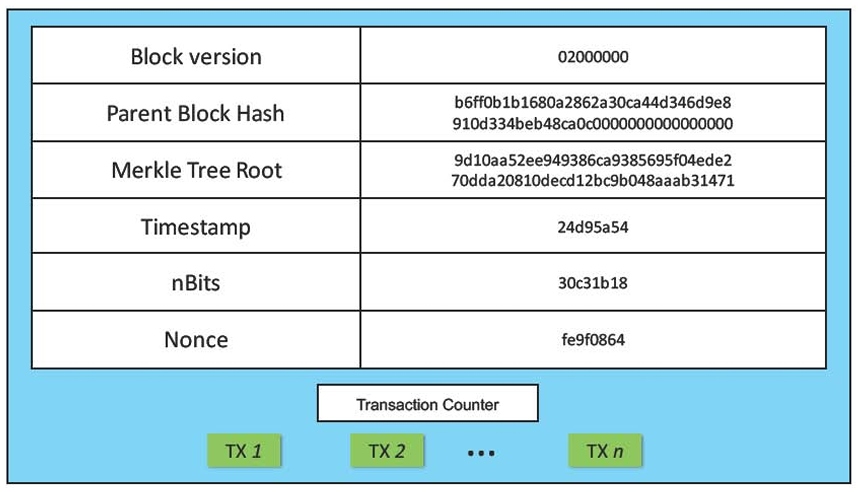
\includegraphics[width=0.7\textwidth]{resources/chapter-2/struktur-block.png}
	\caption{Struktur blok \parencite{zheng2018blockchain}}
	\label{image:struktur-blok}
\end{figure}

\subsection{Karakteristik Blockchain}
\label{subsec:karakteristik-blockchain}

Implementasi dari Blockchain memunculkan karakteristik dari Blockchain itu sendiri. Karakteristik ini dapat muncul secara inheren dari sistem dasar di mana Blockchain dibangun, ataupun muncul karena implementasi spesifik Blockchain. Beberapa karakteristik penting Blockchain \parencite{aimar2023extraction}:

\begin{itemize}
	\item \textit{Decentralized}: Tidak ada sebuah entitas terpusat yang mengontrol jaringan. Seluruh \textit{participants} mengikuti protokol yang berlaku dan memiliki kontrol yang sama.
	\item \textit{Distributed}: Komputasi dilakukan pada sejumlah \textit{node} atau komputer yang berbeda, yang tersebar dan saling berinteraksi melalui sebuah \textit{p2p network}. Kegagalan sebuah mesin seharusnya tidak mengganggu jalannya protokol.
	\item \textit{Immutable}: Tidak memungkinkan untuk mengubah \textit{history} apapun yang sudah tertulis di dalam Blockchain. Setelah sebuah blok divalidasi dan dimasukkan ke dalam Blockchain, tidak dapat dimodifikasi.
	\item \textit{Permissionless}: Semua orang dapat secara aktif berpartisipasi di dalam semua \textit{role} di dalam jaringan tanpa perlu meminta \textit{permission}.
	\item \textit{Permissioned}: Mewajibkan seluruh aktor di dalam jaringan mendapatkan \textit{authorization} secara eksplisit.
	\item \textit{Transparent}: Semua orang dapat secara independen melihat dan mengunduh data dari Blockchain.
	\item \textit{Pseudoanonymous}: \textit{Participants} dalam sebuah \textit{Blockchain network} tidak perlu membuktikan identitas asli mereka. Seluruh aktivitas di dalam jaringan akan disambungkan ke sebuah \textit{address}, bukan identitas asli seseorang.
	\item \textit{Account-based}: data disimpan berdasarkan akun, dan setiap akun memiliki \textit{balance} yang dapat digunakan. Kepemilikan sebuah akun dibuktikan dengan kepemilikan \textit{private key} untuk akun tersebut.
	\item \textit{UTXO-based}: Selain \textit{account-based}, model \textit{UTXO} hanya memiliki konsep dari transaksi. \textit{User} harus membuktikan bahwa mereka memiliki \textit{private key} untuk membuka kunci dari sebuah hasil transaksi untuk menggunakan \textit{balance} yang dimiliki. \textit{Balance} dari seorang \textit{user} adalah penjumlahan seluruh nilai dari hasil transaksi yang dapat dibuka dan digunakan.
\end{itemize}

\subsection{Ethereum}
\label{subsec:ethereum}

Ethereum adalah sebuah platform berbasis Blockchain untuk membangun aplikasi terdesentralisasi dan Smart Contracts, dengan serangkaian \textit{tradeoffs} yang berbeda. Dikembangkan oleh Vitalik Buterin pada tahun 2015, Ethereum mengembangkan konsep dasar Blockchain dengan menambahkan sebuah bahasa pemrograman \textit{Turing-complete} untuk mengembangkan Smart Contracts, yang dijalankan di dalam Ethereum Virtual Machine (EVM). Ethereum Virtual Machine (EVM) adalah sebuah lingkungan eksekusi untuk Smart Contracts di Ethereum, yang memungkinkan kode berjalan di seluruh jaringan Ethereum secara terdistribusi. Bahasa pemrograman bawaan Ethereum yang \textit{Turing-complete} adalah Solidity, yang digunakan untuk menulis Smart Contracts di Ethereum. Solidity adalah bahasa dengan paradigma berorientasi objek, seluruh program Smart Contract akan dikompilasi menjadi sebuah \textit{byte-code}, dalam kasus ini menjadi bentuk EVM Bytecode, dan spesifikasinya dituliskan pada sebuah Application Binary Interface (ABI). Dengan bahasa pemrograman yang \textit{Turing-complete} dan mekanisme eksekusi yang terjamin dengan EVM, Ethereum memberikan kemampuan bagi pengembang untuk mengembangkan sebuah aplikasi yang terdesentralisasi, yang disebut juga sebagai \textit{dApps}, dimana kode dan data disimpan di dalam Blockchain, sehingga mendapatkan karakteristik bawaan dari karakteristik Blockchain \parencite{buterin2013ethereum}.

\subsubsection{ABI}
\label{subsubsec:abi}

\begin{figure}[ht]
  \centering
  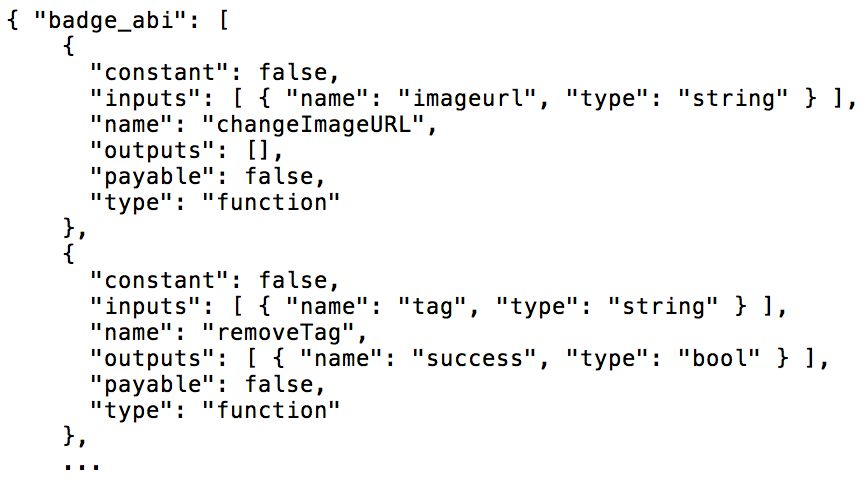
\includegraphics[width=0.7\textwidth]{resources/chapter-2/smart-contract-abi.jpg}
  \caption{Contoh ABI dari sebuah Smart Contract \parencite{third2017linked}}
  \label{image:abi-example}
\end{figure}

Application Binary Interface (ABI) adalah sebuah konvensi yang mendefinisikan aspek-aspek kode yang dihasilkan selama kompilasi, seperti representasi data, penggunaan register, dan konvensi pemanggilan fungsi \parencite{sciencedirect2024}. Dalam konteks Smart Contracts yang ditulis dengan bahasa Solidity dan dikompilasi, hasil dari kompilasinya akan berbentuk EVM Bytecode untuk dieksekusi di dalam EVM, disertai dengan ABI yang mendefinisikan Smart Contract tersebut, seperti pada gambar \ref{image:abi-example}.

\subsubsection{Decentralized Applications (dApps)}
\label{subsubsec:dapps}

Decentralized Applications (dApps) adalah sebuah aplikasi yang berjalan di atas infrastruktur Blockchain dengan memanfaatkan Smart Contracts untuk menyediakan fungsionalitasnya. Karena dApps berjalan di atas Blockchain, dApps mewarisi sifat-sifat yang inheren dari Blockchain, seperti terdesentralisasi, \textit{immutable}, transparan, dan sifat-sifat lainnya \parencite{investopedia2024}. dApps tidak berbeda dari aplikasi tradisional dari sisi pengguna, perbedaannya hanya terletak pada komputasi dari fungsionalitas yang diberikan oleh dApps dilakukan menggunakan Smart Contracts dan seluruh datanya terletak di dalam Blockchain \parencite{metcalfe2020ethereum}. 

\subsubsection{Etherscan}
\label{subsubsec:etherscan}

Etherscan adalah sebuah \textit{block explorer}, \textit{search engine} untuk pengguna agar dapat dengan mudah melihat, mengonfirmasi, dan memvalidasi transaksi untuk Blockchain Ethereum. Etherscan didirikan oleh Matthew Tan pada tahun 2015, dan berdiri secara independen dari Ethereum Foundation. Etherscan melakukan \textit{indexing} terhadap Blockchain untuk menampilkan informasinya, dimana informasi tersebut digunakan untuk menyediakan API untuk pengembang mengintegrasikan informasi Blockchain Ethereum ke dalam aplikasinya \parencite{etherscan2024}.

\subsection{Layer 2}
\label{subsec:layer-2}

Layer 2 adalah sebuah protokol sekunder yang dibangun di atas Blockchain yang sudah ada. Ide dasarnya adalah membangun sebuah \textit{framework} yang mengatasi transaksi \textit{off-chain} sehingga mereduksi beban dari Blockchain dan mendapatkan kecepatan transaksi yang lebih cepat \parencite{sguanci2021layer}. Terdapat beberapa jenis dari solusi Layer 2:

\begin{enumerate}
	\item \textit{Channels L2}: Membuat sebuah komunikasi \textit{off-chain} dengan \textit{node} lain, baik secara langsung maupun tidak langsung. Transaksi antar \textit{node} yang terhubung akan dikelola di Layer 2, dan hanya melaporkan pada \textit{main chain} untuk pembukaan dan penutupan \textit{channel}.
	\item \textit{Sidechains L2}: Sebuah Blockchain "anak" yang berjangkar pada \textit{main chain} dan berjalan secara paralel dengan \textit{main chain}. Serupa dengan Channels, tetapi dalam Sidechains, \textit{off-chain transaction} berjalan di atas Blockchain juga.
	\item \textit{Rollups L2}: Hanya mengeksekusi \textit{transaction} secara \textit{off-chain}, tetapi selalu melaporkan data tentang \textit{transaction} ke dalam \textit{main chain}. Dibandingkan kedua jenis lainnya, Rollups melaporkan data yang lebih kecil untuk setiap \textit{off-chain state update}.
\end{enumerate}

\newpage